%%%%%%%%%%%%%%%%%%%%%%%%%%%%%%%%%%%%%%%%%%%%%%%%%%%
%% LaTeX book template                           %%
%% Author:  Amber Jain (http://amberj.devio.us/) %%
%% License: ISC license                          %%
%%%%%%%%%%%%%%%%%%%%%%%%%%%%%%%%%%%%%%%%%%%%%%%%%%%

\documentclass[a4paper,11pt]{book}
\usepackage[T1]{fontenc}
\usepackage[utf8]{inputenc}
\usepackage{lmodern}
\usepackage[bottom]{footmisc}
\usepackage{circuitikz}
\usepackage{ctable}
%%%%%%%%%%%%%%%%%%%%%%%%%%%%%%%%%%%%%%%%%%%%%%%%%%%%%%%%%
% Source: http://en.wikibooks.org/wiki/LaTeX/Hyperlinks %
%%%%%%%%%%%%%%%%%%%%%%%%%%%%%%%%%%%%%%%%%%%%%%%%%%%%%%%%%
% hidelinks -- gets rid of those red boxes
% pdftoolbar = false -- Hide the Acrobat toolbar on open
% pdfpagelayout = TwoPageRight -- Default to book mode
\usepackage[hidelinks, pdftoolbar=false, pdfpagelayout=TwoPageRight]{hyperref} 
\usepackage{graphicx}
\usepackage[english]{babel}
\usepackage{amsmath}
%%%%%%%%%%%%%%%%%%%%%%%%%%%%%%%%%%%%%%%%%%%%%%%%%%%%%%%%%%%%%%%%%%%%%%%%%%%%%%%%
% 'dedication' environment: To add a dedication paragraph at the start of book %
% Source: http://www.tug.org/pipermail/texhax/2010-June/015184.html            %
%%%%%%%%%%%%%%%%%%%%%%%%%%%%%%%%%%%%%%%%%%%%%%%%%%%%%%%%%%%%%%%%%%%%%%%%%%%%%%%%
\newenvironment{dedication}
{
   \cleardoublepage
   \thispagestyle{empty}
   \vspace*{\stretch{1}}
   \hfill\begin{minipage}[t]{0.66\textwidth}
   \raggedright
}
{
   \end{minipage}
   \vspace*{\stretch{3}}
   \clearpage
}
%\renewcommand{\arraystretch}{1.1}
\newcolumntype{V}{>{\centering\arraybackslash} m{0.25\linewidth} }
%%%%%%%%%%%%%%%%%%%%%%%%%%%%%%%%%%%%%%%%%%%%%%%%
% Chapter quote at the start of chapter        %
% Source: http://tex.stackexchange.com/a/53380 %
%%%%%%%%%%%%%%%%%%%%%%%%%%%%%%%%%%%%%%%%%%%%%%%%
\makeatletter
\renewcommand{\@chapapp}{}% Not necessary...
\newenvironment{chapquote}[2][2em]
  {\setlength{\@tempdima}{#1}%
   \def\chapquote@author{#2}%
   \parshape 1 \@tempdima \dimexpr\textwidth-2\@tempdima\relax%
   \itshape}
  {\par\normalfont\hfill--\ \chapquote@author\hspace*{\@tempdima}\par\bigskip}
\makeatother


% Book's title and subtitle
\title{\Huge \textbf{Electric Circuits}  \\ \huge An Introduction}
% Author
\author{Robert Brown \\ Darby Hewitt}

% ====================================================================
% ====================================================================

\begin{document}

\frontmatter
\maketitle

%\begin{dedication}
%Dedicated to some cool people.
%\end{dedication}

\tableofcontents
%\listoffigures
%\listoftables

\mainmatter

%\section*{Acknowledgements}
%\begin{itemize}
%\item To Robert and Darby, who are awesome!
%\item To the students, who are awesome!
%\item To circuits, which is awesome!
%\end{itemize}

\chapter*{Preface}
This book is made in reaction to many introductory Electrical Engineering texts, which tend to assume a Sophomore- or even Junior-level understanding of Mathematics.  In contrast, we aim our text at Freshmen, who may or may not have completed Calculus I.


% ---------------------------------------------------------------------
\chapter{Underlying Fundamentals}
\section{Review of Algebra}
The things in this section are parts of mathematics that are critical to success in an introductory Circuits course, but that we assume you already know.  In that vein, this section will not be an in-depth coverage of the topic of Algebra, but rather an overview of the specific topics that you will need.
\subsection*{Isolating Variables}
\subsection*{Simple Systems of Equations}
\subsection*{Trigonometry}
\subsection*{Sine and Cosine Curves}


\section{Units} \label{sec:PrelimUnits}

\subsection*{What is electric charge?}
\begin{itemize}
\item Fundamental property of matter
\item Most matter is neutral on a macroscopic level
\item Atoms are composed of:
  \begin{itemize}
  \item protons, which have a positive charge
  \item electrons, which have a negative charge
  \item neutrons, which do not possess a net charge
  \end{itemize}
\item The charge of an electron is constant and the most fundamental unit of charge.  However, it is very small
\item A more useful unit of charge is the Coulomb, which is equivalent to roughly $6.24\times 10^{18}$ electrons.
\end{itemize}

\subsection*{Current, Voltage, Resistance}
The three concepts we will be most interested in throughout this book are current, voltage, and resistance.

Current is:
\begin{itemize}
\item The amount of charge moving through a region (usually a wire) in a given amount of time.
\item Measured in Amperes -- Coulombs per second (1 A = 1 C/s)
\end{itemize}

Voltage is:
\begin{itemize}
\item The amount of energy present in a given amount of charge
\item Also called ``electric potential''
\item Think about a ball on a hill, which has some potential energy.  In this analogy, the mass of the ball is like the charge of our particle, the height of the hill is the voltage, and the potential energy is the electric energy of the particle.
\item Measured in Volts -- Joules per Coulomb (1 V = 1 J/C)
\end{itemize}

Resistance is:
\begin{itemize}
\item A measure of the amount of energy it takes to get some charge through a circuit element in a certain amount of time
\item Measured in Ohms, which does not have a useful conversion to more basic units
\item Think of a very thin pipe. In order to get water through the pipe, you will need to push harder and harder as the pipe gets thinner (or, alternatively, you will have to push harder in order to get more water through the same pipe).  The pipe has some fluid resistance, just as our circuit elements could have some electric resistance.
\item We will cover this more when we get to Ohm's Law
\end{itemize}

\section{A Word on Graphs}
The first thing you probably think of when you hear the word graph is plugging $y=mx+b$ into your calculator.  For the rest of this book, we'll refer to that concept as a plot.

A graph in a purely mathematical sense is a collection of {\bf nodes} and
{\bf branches}. Nodes are like locations or specific points in space, and
branches are the connections between the nodes (similar to pathways between the various locations).  You can draw a graph of this type as shown in Figure \ref{fig:graphTheory}.

% Figure of Example Graph
\begin{figure}
%  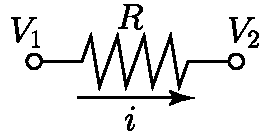
\includegraphics[width=0.5\linewidth]{figures/ohmsLaw}
  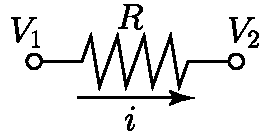
\includegraphics{figures/ohmsLaw}
  \caption{Pictured is a graph, which consists of a number of nodes and branches connecting those nodes.}
  \label{fig:graphTheory}
\end{figure}

We will be using the concept of a graph to talk about electric circuits.


\section{What is a Circuit?}
A circuit is like a graph in that it contains nodes and branches.  For a circuit, a node is any set of locations that is connected by an {\bf ideal wire}.
Charges can pass through ideal wires without any resistance, which means that they aren't losing any energy.  Another way of phrasing it is that the voltage at every point in the wire will be the same: every charge is going to effectively have the same amount of energy in the node.

Branches are any circuit element that is not an ideal wire.  We'll talk later in detail about resistors, voltage sources, and current sources, which are the most common elements used in this class.  Charges that move through these sources will lose or gain energy, and therefore change their voltage.

The final detail about a circuit is that they usually contain a complete loop.  We very rarely have charges accumulate in specific nodes, which means that for charges to move around, they need to move around in a complete circle.  We occasionally have {\bf open circuits}, which do not make a complete loop.  These circuits do not allow any movement of charge, and therefore have no current at all.


\section{Vector Mathematics}
\input{ch_prelim/vector_math}

\section{Complex Numbers}
\begin{itemize}
\item Complex numbers builds on our understanding of vectors
\item If all real numbers can be plotted on a number line, we can draw another number line orthogonal\footnote{perpendicular} to the first to represent imaginary numbers.  A complex number is a point within the plane we created.
\item Complex numbers can be represented in two ways: Cartesian form and polar form
  \begin{itemize}
  \item In Cartesian form, the real and imaginary parts are simply added together, with the imaginary part multiplied with $j$, which is the Circuits name for $\sqrt{\-1}$.  For instance, $1 + j2$ would be a number which is one unit to the right on the Real number line, and two units up on the imaginary number line.
  \item In polar form, a line connecting the point to the origin is defined, and the point is then described using the length of that line and the angle it makes with the Real number line.  $1 + j2$ would have a length of $\sqrt{5}$ and an angle of about 63 degrees or 1.1 rad.  This is commonly represented as $\sqrt{5}e^{j1.1}$ or just $\sqrt{5}\angle{1.1}$
  \item If a number $C$ can be described as $C=x+jy$, it can be converted to polar coordinates ($C=A\angle \theta$) through the following formulas:
    \begin{itemize}
    \item $A = \sqrt{x^2+y^2}$
    \item $\theta = \tan^{-1}\frac{y}{x}$
    \end{itemize}
  \item Likewise, the number can be converted back using these formulas:
    \begin{itemize}
    \item $x = A\cos \theta$
    \item $y = A\sin \theta$
    \end{itemize}
  \end{itemize}
\item Addition is only feasible in Cartesian coordinates.  If you need to add two imaginary numbers in polar form, you should convert both to Cartesian first.
  \begin{itemize}
  \item Take two complex numbers in Cartesian form: $C_1=x_1+jy_1$ and
    $C_2=x_2+jy_2$
  \item The sum of those two numbers is defined as
    $C_1+C_2=(x_1+x_2)+j(y_1+y_2)$
  \item To subtract $C_2$ from the $C_1$, simply negate both $x_2$ and $y_2$:
    $C_1-C_2=(x_1-x_2)+j(y_1-y_2)$
  \end{itemize}
\item Multiplication is feasible in either Cartesian or polar coordinates
  \begin{itemize}
  \item Take two complex numbers in Cartesian form: $C_1=x_1+jy_1$ and
    $C_2=x_2+jy_2$
  \item The product of those two can be written through the FOIL (First, Outer, Inner, Last) method: $C_1\cdot C_2 = x_1x_2 + jx_1y_2 + jx_2y_1 + j^2y_1y_2$
  \item Recognize that $j^2=-1$:
    $C_1\cdot C_2 = x_1x_2 + jx_1y_2 + jx_2y_1 - y_1y_2$
  \item Alternatively, if you have two complex numbers in polar form: $C_1=A_1\angle\theta_1$ and $C_2=A_2\angle\theta_2$
  \item The new amplitude is simply the product of the original amplitudes, and the new angle is the sum of the original angles:
    $C_1\cdot C_2 = C_1C_2\angle(\theta_1+\theta_2)$
  \end{itemize}
\item Division is possible in Cartesian coordinates, but difficult enough that it is much easier to simply convert to polar
  \begin{itemize}
  \item Take two numbers in polar form: $C_1=A_1\angle\theta_1$ and $C_2=A_2\angle\theta_2$
  \item The new amplitude is the result of the division of the original amplitudes, and the new angle is the result of subtraction of the original amplitudes: $C_1/C_2 = A_1/A_2 \angle(\theta_1 - \theta_2)$
  \end{itemize}
\end{itemize}


\section{Linear Algebra}
The first thing to note is that linear algebra is a huge subject with applications not only in circuit analysis, but also in artificial intelligence, simulation and modeling, signal analysis, and computer graphics, just to name a few.  We will only be scratching the surface by covering matrix/vector algebra and matrix inversion.
\subsection*{What is a Matrix?}
A matrix is simply a collection of numbers in an array of a specific size.
For instance, a 2x3 matrix could be written as follows:
\begin{equation*}
  A = \left[
    \begin{tabular}{ccc}
      2 & 1 & -4 \\
      $\pi$ & $2/9$ & 14
    \end{tabular}
    \right]
\end{equation*}
Note that the first number in the size refers to the width or the number of columns of the matrix.  The second refers to the height or the number of rows.

Vectors, by contrast, will always have one of their dimensions that has a length of 1.  A {\bf row vector} would have a size of Nx1, while a {\bf column vector} would have a size of 1xN.
\begin{align*}
  x_{row} =& \left\{\begin{tabular}{ccc} 20 & $\sqrt{2}$ & 0.2 \end{tabular}\right\} &
  x_{col} =& \left\{\begin{tabular}{c} 5 \\ $e^2$ \\ 2 \end{tabular}\right\}
\end{align*}

A {\bf scalar} is a normal number that we are used to working with.  It could be defined as a matrix with a size of 1x1.

\subsection*{Matrix/Vector Algebra}
%% Addition/Subtraction
Once we have some matrices and vectors defined, we can start performing some mathematical operations on them.  First, we have addition/subtraction.  The most important thing to note is that the matrices we use MUST have the same size for us to add or subtract them.  

%% Transpose
Since matrices and vectors have some size and shape to them, we have the ability to move around the numbers inside them.  The operator that does this is known as the {\bf transpose} operator.  Transposing the matrix $A$ from before results in:
\begin{equation*}
  A^T = \left[
    \begin{tabular}{cc}
      2 & $\pi$ \\
      1& $2/9$ \\
      -4 & 14
    \end{tabular}
    \right]
\end{equation*}
Looking at each column, the values come from the original rows.

%% Matrix Vector Multiplication
Multiplication is a bit trickier.  In order to multiply two matrices, the number of rows of the first matrix must match the number of columns for the second matrix.  Also, some of the normal rules of scalar multiplication ($a b = b a$) are slightly modified ($A B = B^T A$)

\subsection*{Writing Systems of Equations Using Linear Algebra}

\subsection*{Matrix Inversion}


\section{Computer Resources - Matlab}
\subsection*{Setting up Matlab/Octave}
\subsection*{Using Matlab to Solve Problems}
\section{Computer Resources - Python}
\subsection*{Setting up Python}
\subsection*{Using Python to Solve Problems}

%%%%%%%%%%%%%%%%%%%%%%%%%%%%%%
\part{DC Circuit Analysis}
%%%%%%%%%%%%%%%%%%%%%%%%%%%%%%

% --------------------------------------------------------------------
\chapter{The First Laws}

\section{Ohm's Law on a Single Resistor}
Ohm's Law describes the amount of energy it takes to push some amount of charge through a resistor.  A reasonable analogy is a ball moving quickly as it approaches a patch of mud.  It starts off with some amount of kinetic energy, then as it moves through the mud, it starts to slow down, losing some portion of the kinetic energy it has, until it clears the puddle.

Unfortunately, our analogy breaks down a bit, since our electrons are moving at the same speed the entire time.  We are not siphoning off the kinetic energy of the electrons, but rather the energy stored in the electrical potential, or voltage.

Ohm's Law states that the voltage drop {\it over} a resistor is proportional to both the resistance, $R$, and the current {\it through} the resistor:
\begin{equation}
  \Delta V = iR
\end{equation}

There is emphasis placed on the words {\it over} and {\it through} due to how we measure the voltage and current in a resistor for Ohm's Law.  We do not care about the voltage at any one place, but rather only the change between the two ends.  Likewise, whatever current is present at any point on the resistor will be present for all of it.  Neither occurs at a single point, but rather describes the entire resistor.

% Figure of Resistor for Ohm's Law
\begin{figure}
   \centering
%  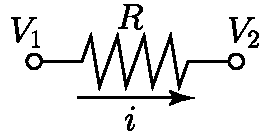
\includegraphics[width=0.5\linewidth]{figures/ohmsLaw}
  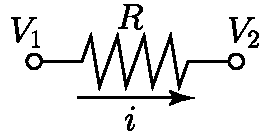
\includegraphics{figures/ohmsLaw}
  \caption{$\Delta V = V_1 - V_2$ for the circuit above, since energy is lost as charge passes through the resistor.}
  \label{fig:ohmsLaw}
\end{figure}

Looking at Figure \ref{fig:ohmsLaw}, you can see that we have labeled the two voltages on either side.  When we apply these voltages to $\Delta V$, we should always start on the tail end of our current (that is, the direction our current is coming from) and end on the head.  

Looking back to the pipe analogy from section \ref{sec:PrelimUnits}, $\Delta V$ is the loss of energy, $i$ is the flow rate through the thin pipe, and $R$ is how hard it is to get through the pipe.  More flow, whether fluid or electric, is more loss of energy, and a smaller pipe or larger resistance also means more loss.

\section{Ohm's Law on a Simple Circuit} \label{sec:FL_simpleCircuit}

\section{Kirchoff's Current Law}

\section{Watt's Law}

\section{Incorporating Computation - Plotting}
% --------------------------------------------------------------------
\chapter{Equivalent Circuits}
This chapter introduces the concept of an equivalent circuit.  Two equivalent circuits share common values of voltage/current at a point of interest, usually the source.  In this chapter, we will simplify complex resistive circuits down to the simplest version (such as those analyzed in Section \ref{sec:FL_simpleCircuit}).  Once simplified, we will expand them again through methods known as voltage division and current division to find the current through each element and the voltage at each node.

\section{Resistors in Series}
First, lets go over in a bit more detail what we mean by {\it \bf series}. Two elements are in series if and only if:
\begin{itemize}
\item Those elements share a common node
\item No other elements share the same node
\end{itemize}

% Figure of Resistors in Series
\begin{figure}
\centering
%  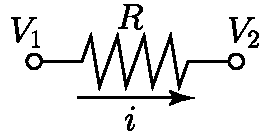
\includegraphics[width=0.5\linewidth]{figures/ohmsLaw}
  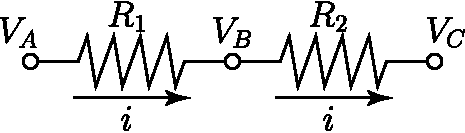
\includegraphics{figures/resistorSeries}
  \caption{The two resistors above are the only circuit elements connected to node $B$, which means that any current from node $A$ to $B$ will also have to travel from $B$ to $C$.}
  \label{fig:resistorSeries}
\end{figure}
%% \begin{circuitikz} \draw[scale=1]
%%   (0, 0) node[label={$V_A$}] {}
%%   to[resistor, l=$R_1$, o-o] (2, 0) node[label={$V_B$}] {}
%%   to[resistor, l=$R_2$, o-o] (4,0) node[label={$V_C$}] {}
%%   ;
%% \end{circuitikz}


In this case, there is exactly one path for current to follow through both resistors.  Because of this, we can write the following:
\begin{eqnarray}
  \label{eq:series1} \Delta V_1 &=& V_A-V_B = i R_1 \\ 
  \label{eq:series2} \Delta V_2 &=& V_B-V_C = i R_2 
\end{eqnarray}

Now, our goal is to create simpler circuit which has the same characteristics as seen by nodes $A$ and $C$. The only way to get simpler is to have a single circuit between nodes $A$ and $C$ with a resistance which we still need to determine.

We want our new circuit to have the following characteristics:
\begin{itemize}
\item The current through the new resistor should still be the $i$ that passes through $R_1$ and $R_2$
\item The voltage difference across the new resistor should be $V_A - V_C$
\end{itemize}

We can fulfill those two requirements by summing equations \ref{eq:series1} and \ref{eq:series2}:
\begin{equation} \label{eq:series3}
\Delta V_1 + \Delta V_2 = V_A - V_C = i (R_1 + R_2)
\end{equation}

Equation \ref{eq:series3} essentially states that we can replace both resistors with a single resistor that has a resistance
\begin{equation} \label{eq:seriesEquivalent}
R_{EQ}=R_1+R_2.
\end{equation}

\section{Resistors in Parallel}
\begin{itemize}
\item Definition of parallel - recap
\item Derivation of parallel resistance
  \begin{itemize}
  \item Voltage constant across both resistors
  \item Equivalent resistance should sum current while maintaining voltage
  \item End result: $R_{EQ}=R_1\cdot R_2 / (R_1 + R_2)$
  \end{itemize}
\end{itemize}


%% I'm in favor of omitting this section in favor of emphasizing the
%%  definitions of parallel and series
%\section{Reorganizing Complicated Circuits}
%\begin{itemize}
\item Recognizing elements in series or parallel is often the most difficult part of simplifying circuits
\item Reorganizing the circuits can help in this process
\item The process looks something like this:
  \begin{itemize}
  \item Determine the number of nodes and label each
  \item Draw each of the nodes in a line
  \item Identify connections between the nodes
  \item Draw each of those connections, making connections between adjacent nodes close to the center line, and connection between more distant nodes further from the center line
  \item Elements in series and parallel are now easier to identify
  \end{itemize}
\end{itemize}


\section{Wye-Delta Transform}
\input{ch_eqCircuits/wyeDelta}
\section{Using Voltage Division}
\input{ch_eqCircuits/voltageDivision}
\section{Using Current Division}
\input{ch_eqCircuits/currentDivision}
\section{Circuit Shorthand}
\input{ch_eqCircuits/shorthand}
\section{Incorporating Computation - $R_1||R_2$ Function}
\input{ch_eqCircuits/computation}

% --------------------------------------------------------------------
\chapter{Extra Uses for Voltage Dividers}
\section{Maximum Power Transfer}
\begin{itemize}
\item Sources/loads
\item If we know all the information about the source, we can calculate the power drawn by any load
  \begin{itemize}
  \item Use voltage division to find voltage $V_0 = V_s \frac{R_0}{R_s+R_0}$
  \item $P_0=V_0^2/R_0$
  \end{itemize}
\item When we ask the question ``What load will draw the maximum power?'', we need to dip into Calculus
  \begin{itemize}
  \item The maximum of a function $f(x)$ occurs when the derivative $f'(x)$ goes to zero
  \item Our function is $\displaystyle P_0(R_0)=\left( V_s \frac{R_0}{R_s+R_0}\right)^2 \cdot \frac{1}{R_0}$
  \item We need to solve $\displaystyle P_0'(R_0) = V_s^2 \cdot \frac{(R_s^2+R_0^2)-R_0\cdot 2 R_0}{(R_s^2+R_0^2)^2} = 0$
  \item A little bit of algebra tells us that this occurs when $R_0 = \pm R_s$
  \item Only positive $R_0$ makes sense, so $R_0=R_s$ for maximum power
  \end{itemize}
\item Once we know where maximum power occurs, it is trivial to find the value of the maximum power in terms of known values $V_s$ and $R_s$
  \begin{itemize}
  \item Use voltage division to find $V_0=V_s/2$
  \item Use the power equation to get $P_0=V_s^2/(4 R_s)$
  \end{itemize}
\item Other interesting notes:
  \begin{itemize}
  \item Why doesn't higher voltage across $R_0$ lead to higher power? If we increase $R_0$ past the value of $R_s$, we do increase the value of voltage over $R_s$, but we decrease the current through both resistors, which ends up decreasing the power absorbed by $R_0$.
  \item If that's the case, why don't we decrease $R_0$?  Well, decreasing $R_0$ does indeed increase the current through both resistors, but only to a point (our current can't go higher than $V_s/R_s$).  Decreasing $R_0$ also has the effect of decreasing the voltage over the resistor, and the total effect is to decrease the power absorbed by the load.
  \item It turns out that $R_0=R_s$ is the sweet spot, as you can see by the plot shown in Figure \ref{fig:maxPower}
  \end{itemize}
\end{itemize}

% Plot of Power in the region of R0 = Rs
\begin{figure}
   \centering
%  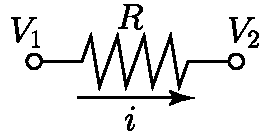
\includegraphics[width=0.5\linewidth]{figures/ohmsLaw}
  
\includegraphics{figures/toDo}
  \caption{This plot shows the power absorbed by the load resistor as its resistance $R_0$ is changed.  The $x$-axis has been normalized by $R_s$, and the $y$-axis has been normalized by the maximum power, $V_s/R_s^2$.}
  \label{fig:maxPower}
\end{figure}

\section{Nonlinear Circuit Elements}
\section{Incorporating Computation - Graphical Analysis}
% --------------------------------------------------------------------
\chapter{Operational Amplifiers}
\section{What is an Op-Amp?}
\begin{itemize}
\item Op-Amp stands for Operational Amplifier
\item An amplifier is a device that receives an input and sends an output that is proportional to the input
\end{itemize}

\section{Golden Rules}
\subsection*{Input Current is Zero ($i_+=i_-=0$)}
Looking back at our simple model of the Op-Amp, this stems from our assumption that $R_{in}$ is very large.  Lets assume that the input voltage is in a normal range (something like 5-20 V) and that $R_{in}$ is about 1 G$\Omega$.  In that case, the current through the resistor looks something like
\begin{equation*}
  i_{in}=V_{in}/R_{in}=20 \text{V} / 1\text{G}\Omega = 20 \text{nA}.
\end{equation*}
  That is, admittedly, not zero.  However, if we try to account for that error in a normal circuit (one in which the current is measured in mA), the error we get from neglecting it is on the order of 0.01\%.
\subsection*{ Voltage is Equivalent if Feedback is Present ($V_-=V_+$)}


\section{Analyzing Circuits with Op-Amps}

%%%%%%%%%%%%%%%%%%%%%%%%%%%%%
\part{Alternating Current}
%%%%%%%%%%%%%%%%%%%%%%%%%%%%%

% --------------------------------------------------------------------
\chapter{AC Circuits}
\begin{itemize}
\item Description of time-varying current/voltage in general
\item Specification of sinusoidal time-varying current/voltage
  \begin{itemize}
  \item Frequency
  \item Phase angle
  \end{itemize}
\item Definition of lagging/leading
  \begin{itemize}
  \item Difference between phase angles
  \item Recognition that there is no lead/lag for resistive circuits
  \end{itemize}
\item Solution of $\Delta V=iR$ for purely resistive circuits
\end{itemize}

\section{Phasor Notation}
\begin{itemize}
\item Callback to Euler's Formula (back to Ch. 1)
\item $\cos{\omega t + \phi} = \Re \left\{ e^{j\omega t}e^{j\phi} \right\}$
\item Give an amplitude associated with the circuit:
  $\Re \left\{ A e^{j\omega t}e^{j\phi} \right\}$
\item Hide $e^{j\omega t}$, since we typically only deal with one frequency at a time:
  $\Re \left\{ A e^{j\phi} \right\}$
\item Hide the $\Re$, since we know we want the real part:
  $Ae^{j\phi}$
\item Replace $e^{j\phi}$ with the simpler $\angle\phi$:
  $A\angle\phi$
\item Now you have phasor notation
\end{itemize}

\section{Capacitors}
\begin{itemize}
\item Capacitors are energy storage devices that store up electric charge
\item Most simply two plates in parallel with a gap filled with some non-conducting material
\item Amount of charge stored is proportional to voltage: $q=CV$
\item $C$ is the {\bf capacitance} of the capacitor, and is measured in Farads (F)
\item Current is change in charge per change in time: $i = \frac{\Delta q}{\Delta t}$
\item Can be analyzed through Calculus ($i = \frac{d q}{d t}$)
\item Using Euler's Formula and Calculus, it is possible to reduce $q=CV$ to $\Delta V=iZ_C$, where $Z_C=\frac{1}{j\omega C}$
\item Again using Calculus, it is possible to find that $E_C=\frac{1}{2}CV^2$
\item Full mathematical details in Appendix (not yet!)
\end{itemize}

\section{Inductors}
\begin{itemize}
\item Inductors are energy storage devices that create a magnetic field
\item Typically composed of a coil of wire surrounding a ferromagnetic core
\item Magnetic fields resist change, and the change in the magnetic field per change in time results in a voltage difference (Faraday's law): $\Delta V = -\frac{d \Phi}{d t}$
\item The magnetic field generated is proportional to the current through the inductor: $\Phi = Li$
\item $L$ is the inducatance of the inductor, and is measured in Henrys (H)
\item Through the same methods as capacitors, it is possible to reduce $\Delta V = -\frac{d \Phi}{d t}$ to $\Delta V = i Z_L$, where $Z_L=j\omega L$
\item The energy stored in the inductor is $E_L=\frac{1}{2}Li^2$
\item Full mathematical details in Appendix (not yet!)
\end{itemize}

\section{Equivalent Impedance and Ohm's Law}

\begin{itemize}
\item Impedances of each component summarized in
  Table \ref{tab:impedanceSummary}
\item Equivalent impedance evaluated exactly as equivalent resistance:
  $Z_{series} = Z_1+Z_2$, $Z_{parallel}=\frac{Z_1\cdot Z_2}{Z_1+Z_2}$
\item Several shortcuts can be used for like elements:
  \begin{itemize}
  \item $C_{parallel}=C_1+C_2$, $C_{series} = \frac{C_1\cdot C_2}{C_1+C_2}$
  \item $L_{series} = L_1+L_2$, $L_{parallel} = \frac{L_1\cdot L_2}{L_1+L_2}$
  \end{itemize}
\item Ohm's Law works in AC exactly like it does in DC, just replace $R$ with $Z$: $\Delta V$ = $I Z$
\end{itemize}
\ctable[
  cap = Impedance Element Summary,
  caption = A Summary of Elements Which Provide an Impedance,
  label = tab:impedanceSummary,
  pos = h
]{lVVV}{
  \tnote{Typical ceramic capacitors. Electrolytic capacitors have larger capacitance.}
  }{
  \FL
  & Capacitor                     & Inductor                & Resistor                     \\
  \midrule \vspace{-1em}\\ \vspace{-0.25em}
  Symbol
  & 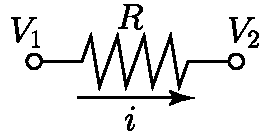
\includegraphics[height=30pt]{figures/ohmsLaw} 
  & 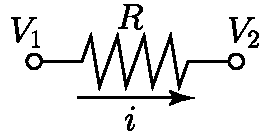
\includegraphics[height=30pt]{figures/ohmsLaw} 
  & 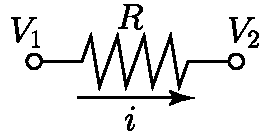
\includegraphics[height=30pt]{figures/ohmsLaw} \\
  Unit & Farad (F) & Henry (H) & Ohm ($\Omega$)      \\ \vspace{0.25 em}
  Typical Values
  & 0.1 pF -- 0.5 mF\tmark
  & 0.1 $\mu$H -- 10 mH
  & 10 $\Omega$ -- 1 G$\Omega$ \\ \vspace{0.5 em}
  Impedance
  & $\displaystyle Z_C=\frac{1}{j \omega C}$
  & $\displaystyle Z_L = j \omega L$
  & $\displaystyle Z_R = R$                    \\ 
  Energy Storage
  &  $\displaystyle E_C = \frac{1}{2} CV^2$
  & $\displaystyle E_L = \frac{1}{2}Li^2$
  & N/A 
\LL
}



% --------------------------------------------------------------------
\chapter{AC Power}
\section{Watt's Law for AC}
\begin{itemize}
\item Power for AC circuits looks a little different than for DC
\item $p(t) = v(t)*i(t)$ %, but we usually want some sort of average power
\item Plot voltage, current, and power for a resistive load
\item Do the same for a capacitive, inductive load
\item Again for resistive + capacitive
\item Find average power through integration
\end{itemize}

\section{Average Power}
\begin{itemize}
\item Helpful to introduce some additional ways of talking about amplitude
  \begin{itemize}
  \item The amplitude we've been using is the {\bf peak} amplitude.  As an example, the peak voltage would be written as $V_p$.
  \item Another useful amplitude is the {\bf peak-to-peak} amplitude.  This measures the total distance between peaks, and is typically written as $V_{pp}$.  The peak-to-peak voltage is twice the peak amplitude.
  \item Finally, we have the {\bf RMS} amplitude.  RMS stands for root-mean-square, which refers to the method used to obtain it (find more information in the Appendix). For sinusoidal voltage, $V_{RMS}=\frac{1}{\sqrt{2}}V_p$.  For non-sinusoids, the RMS voltage will be different.
    %$V_{RMS} = \sqrt{\frac{1}{T} \int_0^T v(t)^2 dt}$.  
  \end{itemize}
\item The RMS voltage and current are directly used in finding the power.  Watt's law for AC gives that the average power is the product of the root-mean-square voltage and current multiplied by the cosine of the phase offset between the two: $P_{avg}=V_{RMS}I_{RMS}\cos(\phi_V-\phi_I)$.  Translated to peak amplitudes (which we normally use), $P_{avg}=\frac{1}{2}V_pI_p\cos(\phi_V-\phi_I)$
\end{itemize}

\section{Complex Power}
\begin{itemize}
\item Definition: $S=VI^*$
\item What does Imaginary Power mean?  Why does it matter?
\item Power factor: $pf = \cos(\phi_Z)$
\item Calculating complex power for simple circuits
\end{itemize}

\section{Power Factor Correction}
\input{ch_ACPower/powerFactorCorrection}
\section{Maximum Power for AC Circuits}
\input{ch_ACPower/ACmaxPower}
% --------------------------------------------------------------------
\chapter{Passive Filters}
\section{Frequency Response}
\begin{itemize}
\item General circuit (right now a highpass)
\item Plotting (linear -> semilog -> loglog)
\item RC and RL circuits (analysis and design)
\begin{itemize}
\item Highpass filter
\item Lowpass filter
\end{itemize}
\item RLC circuits (analysis and design)
\begin{itemize}
\item Bandpass
\item Bandstop/notch
\item Second-order Highpass
\item Second-order Lowpass
\end{itemize}
\item RCRC circuits (Commentary on ease of construction)
\end{itemize}


When we talk about analyzing filters, what we mean is how does the output voltage respond to different frequencies.  We call this the {\bf freqeuncy response} of the circuit.  In practice, this results in solving for the output voltage while keeping $\omega$ a variable.  Figure \ref{fig:CircuitRC} shows an AC source connected to a capacitor and resistor in series.

\begin{figure}
   \centering
%  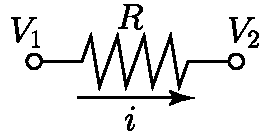
\includegraphics[width=0.5\linewidth]{figures/ohmsLaw}
  
\includegraphics{figures/toDo}
  \caption{A simple circuit composed of a source and two components.}
  \label{fig:CircuitRC}
\end{figure}

Our goal here is to find the frequency response of the output voltage.  We know that $Z_C=\frac{1}{j\omega C}$ and $Z_R = R$.  From voltage division, we obtain the following:
\begin{equation} \label{eq:CircuitLC}
  V_{out} = V_s \frac{R}{R + \frac{1}{j \omega C}}
\end{equation}

Simplified, we can rewrite this as:
\begin{equation}
  \frac{V_{out}}{V_s}=\frac{j \omega RC}{1 + j\omega RC}
\end{equation}

At this point, we either feed this into a program, which can calculate the response over a wide variety of $\omega$ values, or we look into some limits. Specifically, we'd like to find the limit as $\omega$ approaches zero and infinity.

\begin{align}
  \lim_{\omega \to 0} \frac{j \omega RC}{1 + j\omega RC} &= \frac{j (0) RC}{1 + j (0) RC} = 0 \\
  \lim_{\omega \to \infty} \frac{j \omega RC}{1 + j\omega RC} &= \frac{j RC}{j RC} = 1
\end{align}

If we want to plot the response by hand, we need to look at one more value, typically called the {\bf breakpoint frequency}, $\omega_b$.  This is defined as the freqency at which the magnitude of impedance of the two components are equal ($|Z_R| = |Z_C|$):
\begin{align*}
  \left|\frac{1}{j\omega_b C}\right| &= R &
  \frac{1}{\omega_b C} &= R &
  \omega_b &= \frac{1}{RC}
\end{align*}
  
If we plug this back into our frequency response, we find the following:
\begin{align*}
  \frac{V_{out}}{V_s}&=\frac{j RC\left(\frac{1}{RC}\right)}{1 + j RC \left(\frac{1}{RC}\right)} \\
  \frac{V_{out}}{V_s}&=\frac{j}{1+j} \\
  \left|\frac{V_{out}}{V_s}\right|&=\frac{|j|}{|1+j|}=\frac{1}{\sqrt{2}}
\end{align*}

In fact, this is an equivalent definition of the breakpoint frequency.  Our breakpoint occurs when the magnitude of our frequency response is exactly $\sqrt{2}$.

Let's do the other option.  If we have access to a computer, we can plot the amplitude and phase angle of the frequency response as seen in Figure \ref{fig:freqResponseLinear}.  This plot is useful, but we can change our axes to see things a little cleaner.

\begin{figure}
   \centering
%  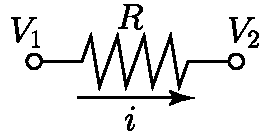
\includegraphics[width=0.5\linewidth]{figures/ohmsLaw}
  
\includegraphics{figures/toDo}
  \caption{The frequency response of the circuit using linear axes.}
  \label{fig:freqResponseLinear}
\end{figure}

Figure \ref{fig:freqResponseLog} shows a log-log plot of the frequency response. In this plot, $\omega$ is replaced in the $x$-axis by $\log(\omega)$ and $\left|\frac{V_{out}}{V_s}\right|$ is replaced by $\log\left(\left|\frac{V_{out}}{V_s}\right|\right)$.  Doing so, the behaviour of the circuit stands out very clearly.  Note that the phase angle $\phi$ did not change between Figures \ref{fig:freqResponseLinear} and \label{fig:freqResponseLog}.

\begin{figure}
   \centering
%  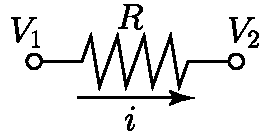
\includegraphics[width=0.5\linewidth]{figures/ohmsLaw}
  
\includegraphics{figures/toDo}
  \caption{The frequency response of the circuit using logarithmic axes.}
  \label{fig:freqResponseLog}
\end{figure}

So what's happening?  Starting at high frequencies, the response is fairly constant until you hit the break point, and then it drops off logarithmically as you decrease the frequency.  To describe this, we say that we allow high frequencies to {\it pass through}.  In shorter terms, this is a {\bf highpass filter}.

\section{Two-element Filters}
To start off, let's analyze some filters that we can create with two elements.  The first of these will combine a resistor and a capacitor, as shown in Figure \ref{fig:RC_highpass}.

\begin{figure}
   \centering
%  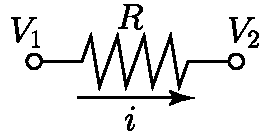
\includegraphics[width=0.5\linewidth]{figures/ohmsLaw}
  
\includegraphics{figures/toDo}
  \caption{A simple circuit composed of a source and two components.}
  \label{fig:RC_highpass}
\end{figure}

\section{Second Order Filters}
\begin{itemize}
\item Highpass filter
\item Lowpass filter
\item Bandpass filter
\item Bandstop filter
\item Composite filters
\end{itemize}


% --------------------------------------------------------------------
\chapter{Active Filters}
\section{Op-Amps in AC}
\begin{itemize}
\item Recap inverting amplifier: $G(\omega) = -Z_f/Z_s$
\item Recap non-inverting amplifier: $G(\omega) = 1+Z_f/Z_s$
\item General construction rules (avoiding $Z_f \rightarrow \infty$ and $Z_s \rightarrow 0$)
\end{itemize}

\section{First Order Filters}
\begin{itemize}
\item Highpass filter
  \begin{itemize}
  \item Add a capacitor in series with $R_s$ or an inductor in parallel with $R_f$
  \item Maximum amplitude will be $R_f/R_s$
  \end{itemize}
\item Lowpass filter
  \begin{itemize}
  \item Add an inductor in series with $R_s$ or a capacitor in parallel with $R_f$
  \item Maximum amplitude will be $R_f/R_s$
  \end{itemize}
\item Redrawing circuits with equivalent components at $\omega \rightarrow 0$ and $\omega \rightarrow \infty$ limits
\end{itemize}

\section{Second Order Filters}
\begin{itemize}
\item Highpass filter
\item Lowpass filter
\item Bandpass filter
\item Bandstop filter
\item Composite filters
\end{itemize}


%%%%%%%%%%%%%%%%%%%%%%%%%%%%%%%%%%%
\part{Analysis of Circuit Networks}
%%%%%%%%%%%%%%%%%%%%%%%%%%%%%%%%%%%
% --------------------------------------------------------------------
\chapter{Superposition}

% --------------------------------------------------------------------
\chapter{Node Voltage Method}
\section{Kirchoff's Current Law Revisited}
\section{Using the Node Voltage Method}
\subsection*{Writing KCL}
\subsection*{Converting to Voltage with Ohm's Law}
\subsection*{Dealing with Voltage Sources}
\subsection*{Dealing with Dependent Sources}
\section{Incorporating Computation - Linear Algebra}
% --------------------------------------------------------------------
\chapter{Mesh Current Method}
\section{Mesh Currents vs. Branch Currents}
\section{Kirchoff's Voltage Law}
\section{Incorporating Computation - Linear Algebra}
%--------------------------------------------------------------------
\chapter{Thevenin and Norton Equivalent Circuits}
\section{Circuit Loads}
\section{Determining Thevenin Resistance}
\section{Determining Thevenin Voltage}
\section{Determining Norton Current}

\end{document}
